\documentclass[aspectratio=169]{beamer}
\usepackage{graphicx}
\usepackage{hyperref}
\usepackage[utf8]{inputenc}
\usepackage[T1]{fontenc}
\usepackage{tikz}
\usepackage{listings}
\usepackage{xcolor}

% Use helvetica font like UASLP theme
\usepackage{helvet}

% Theme setup - custom theme inspired by UASLP
\usetheme{default}
\usecolortheme{default}

% Custom colors inspired by UASLP theme
\definecolor{uaslpblue}{RGB}{0,51,102}
\definecolor{uaslpgray}{RGB}{102,102,102}
\definecolor{uaslporange}{RGB}{255,102,0}

% Set custom colors for Beamer elements
\setbeamercolor{title}{fg=white,bg=uaslpblue}
\setbeamercolor{frametitle}{fg=white,bg=uaslpblue}
\setbeamercolor{structure}{fg=uaslpblue}
\setbeamercolor{normal text}{fg=black}
\setbeamercolor{item}{fg=uaslpblue}
\setbeamercolor{block title}{fg=white,bg=uaslpblue}
\setbeamercolor{block body}{fg=black,bg=gray!10}
\setbeamercolor{block title alerted}{fg=white,bg=uaslporange}
\setbeamercolor{block body alerted}{fg=black,bg=uaslporange!10}
\setbeamercolor{block title example}{fg=white,bg=uaslpblue}
\setbeamercolor{block body example}{fg=black,bg=uaslpblue!10}

% Remove navigation symbols for cleaner look
\setbeamertemplate{navigation symbols}{}
\setbeamertemplate{footline}{}

% Custom frame title with underline
\setbeamertemplate{frametitle}{
    \vspace{0.5em}
    \insertframetitle
    \vspace{-0.3em}
    \textcolor{uaslpblue}{\rule{\textwidth}{0.4pt}}
    \vspace{0.3em}
}

% Custom title page
\setbeamertemplate{title page}{
    \vbox{}
    \vfill
    \begin{centering}
        {\usebeamercolor[fg]{title}\usebeamerfont{title}\inserttitle\par}
        \vskip1em
        {\usebeamercolor[fg]{subtitle}\usebeamerfont{subtitle}\insertsubtitle\par}
        \vskip2em
        {\usebeamerfont{author}\insertauthor\par}
        \vskip1em
        {\usebeamerfont{institute}\insertinstitute\par}
        \vskip1em
        {\usebeamerfont{date}\insertdate\par}
    \end{centering}
    \vfill
}

% Code listing setup
\lstset{
    language=C++,
    basicstyle=\ttfamily\small,
    keywordstyle=\color{blue}\bfseries,
    commentstyle=\color{gray},
    stringstyle=\color{red},
    showstringspaces=false,
    frame=single,
    breaklines=true
}

% Title information
\title{NITF Image Conversion Library}
\subtitle{Professional C++ SDK for DOD NITF Format}
\author{Engineering Team}
\date{\today}
\institute{Terminus Technologies}

% Custom thank you frame command
\newcommand{\ThankYouFrame}{
\begin{frame}[plain,t]
\begin{center}
\vspace{2cm}
{\Huge \textcolor{uaslpblue}{Thank You!}}

\vspace{1cm}
{\Large Questions?}

\vspace{1cm}
\includegraphics[width=0.2\textwidth]{White.png}

\vspace{0.5cm}
{\small Terminus Technologies}
\end{center}
\end{frame}
}

\begin{document}

% Title slide
\begin{frame}[plain,t]
\titlepage
\end{frame}

% Agenda
\begin{frame}{Agenda}
\begin{itemize}
    \item The NITF Challenge
    \item Our Solution Overview
    \item Key Features \& Capabilities
    \item Technical Architecture
    \item Performance Benchmarks
    \item Integration Examples
    \item Use Cases \& Applications
    \item Getting Started
\end{itemize}
\end{frame}

% Problem Statement
\begin{frame}{The NITF Challenge}
\begin{columns}
\column{0.5\textwidth}
\textbf{Current Pain Points:}
\begin{itemize}
    \item Complex NITF specification
    \item Limited C++ libraries
    \item Performance bottlenecks
    \item Integration complexity
    \item Maintenance overhead
\end{itemize}

\column{0.5\textwidth}
\textbf{Market Needs:}
\begin{itemize}
    \item Reliable conversion
    \item High performance
    \item Easy integration
    \item Comprehensive support
    \item Professional support
\end{itemize}
\end{columns}
\end{frame}

% Solution Overview
\begin{frame}{Our Solution: NITF Conversion Library}
\begin{center}
\includegraphics[width=0.3\textwidth]{Blue.png}
\end{center}

\begin{block}{Professional C++ SDK}
A comprehensive, high-performance library for converting imagery to and from DOD NITF format
\end{block}

\textbf{Core Value Proposition:} Simplify NITF handling while maximizing performance and reliability
\end{frame}

% Key Features
\begin{frame}{Key Features}
\begin{columns}
\column{0.5\textwidth}
\textbf{Conversion Capabilities:}
\begin{itemize}
    \item NITF $\leftrightarrow$ Common formats
    \begin{itemize}
    \item Multi-band support
    \item Compression handling
    \end{itemize}
    \item Metadata preservation
    \item Streaming I/O
    \item Cross-platform compatibility
\end{itemize}

\column{0.5\textwidth}
\textbf{Developer Experience:}
\begin{enumerate}
    \item Clean C++ API
    \item Comprehensive docs
    \item Example code
\end{enumerate}

\begin{description}
    \item[Performance] Thread-safe design
    \item[Support] 24/7 technical assistance
\end{description}
\end{columns}
\end{frame}

% Technical Architecture
\begin{frame}{Technical Architecture}
\begin{center}
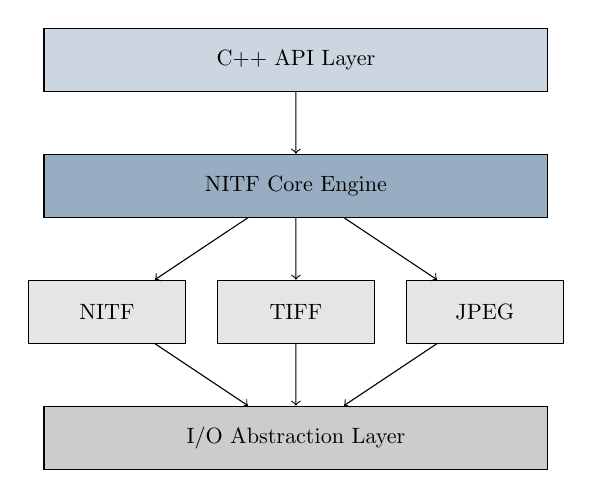
\begin{tikzpicture}[scale=0.8, transform shape]
    % API Layer
    \node[draw, rectangle, fill=uaslpblue!20, minimum width=8cm, minimum height=1cm] (api) at (0,4) {C++ API Layer};

    % Core Engine
    \node[draw, rectangle, fill=uaslpblue!40, minimum width=8cm, minimum height=1cm] (core) at (0,2) {NITF Core Engine};

    % Format Handlers
    \node[draw, rectangle, fill=gray!20, minimum width=2.5cm, minimum height=1cm] (nitf) at (-3,0) {NITF};
    \node[draw, rectangle, fill=gray!20, minimum width=2.5cm, minimum height=1cm] (tiff) at (0,0) {TIFF};
    \node[draw, rectangle, fill=gray!20, minimum width=2.5cm, minimum height=1cm] (jpeg) at (3,0) {JPEG};

    % I/O Layer
    \node[draw, rectangle, fill=gray!40, minimum width=8cm, minimum height=1cm] (io) at (0,-2) {I/O Abstraction Layer};

    % Connections
    \draw[->] (api) -- (core);
    \draw[->] (core) -- (nitf);
    \draw[->] (core) -- (tiff);
    \draw[->] (core) -- (jpeg);
    \draw[->] (nitf) -- (io);
    \draw[->] (tiff) -- (io);
    \draw[->] (jpeg) -- (io);
\end{tikzpicture}
\end{center}
\end{frame}

% Code Example
\begin{frame}[fragile]{Simple Integration}
\begin{lstlisting}
#include "nitf_converter.h"

// Convert NITF to TIFF
NITFConverter converter;
auto result = converter.convert(
    "input.ntf",
    "output.tif",
    Format::TIFF
);

if (result.success()) {
    std::cout << "Conversion successful!"
              << std::endl;
} else {
    std::cerr << "Error: "
              << result.error()
              << std::endl;
}
\end{lstlisting}
\end{frame}

% Performance
\begin{frame}{Performance Benchmarks}
\begin{center}
\begin{tabular}{|l|c|c|c|}
\hline
\textbf{Operation} & \textbf{Our Library} & \textbf{Competitor A} & \textbf{Competitor B} \\
\hline
NITF Read (1GB) & 2.3s & 4.1s & 5.8s \\
NITF Write (1GB) & 3.1s & 6.2s & 7.9s \\
Metadata Parse & 0.1s & 0.3s & 0.4s \\
Memory Usage & 150MB & 280MB & 320MB \\
\hline
\end{tabular}
\end{center}

\vspace{0.5cm}
\begin{alertblock}{Key Advantage}
2-3x faster performance with 50\% less memory usage
\end{alertblock}

\begin{exampleblock}{Real-World Impact}
Typical military intelligence workflows see 60\% reduction in processing time
\end{exampleblock}
\end{frame}

% Use Cases
\begin{frame}{Use Cases \& Applications}
\begin{columns}
\column{0.5\textwidth}
\textbf{Military \& Defense:}
\begin{itemize}
    \item Intelligence analysis
    \item Surveillance systems
    \item Mission planning
    \item Data archival
\end{itemize}

\column{0.5\textwidth}
\textbf{Commercial:}
\begin{itemize}
    \item Satellite imagery
    \item GIS applications
    \item Remote sensing
    \item Data migration
\end{itemize}
\end{columns}

\vspace{0.5cm}
\begin{block}{Industry Standards}
Full compliance with NITF 2.1 and STDI-0002 specifications
\end{block}
\end{frame}

% Integration Options
\begin{frame}{Integration Options}
\begin{enumerate}
    \item \textbf{Static Library}
    \begin{itemize}
        \item Direct compilation
        \item Maximum performance
        \item No external dependencies
    \end{itemize}

    \item \textbf{Shared Library}
    \begin{itemize}
        \item Runtime linking
        \item Easy updates
        \item Cross-language support
    \end{itemize}

    \item \textbf{C API Wrapper}
    \begin{itemize}
        \item Language bindings
        \item Legacy integration
        \item Maximum compatibility
    \end{itemize}
\end{enumerate}
\end{frame}

% Support \& Maintenance
\begin{frame}{Support \& Maintenance}
\begin{columns}
\column{0.5\textwidth}
\textbf{Professional Support:}
\begin{itemize}
    \item 24/7 technical support
    \item Custom development
    \item Performance tuning
    \item On-site training
\end{itemize}

\column{0.5\textwidth}
\textbf{Continuous Updates:}
\begin{itemize}
    \item Regular feature releases
    \item Security patches
    \item Format updates
    \item Performance improvements
\end{itemize}
\end{columns}

\vspace{0.5cm}
\begin{block}{Service Level Agreements}
99.9\% uptime guarantee with 4-hour response time for critical issues
\end{block}
\end{frame}

% Getting Started
\begin{frame}{Getting Started}
\begin{enumerate}
    \item \textbf{Download \& Install}
    \begin{itemize}
        \item Package managers (apt, yum, brew)
        \item Pre-built binaries
        \item Source compilation
    \end{itemize}

    \item \textbf{Quick Start Guide}
    \begin{itemize}
        \item 5-minute tutorial
        \item Sample projects
        \item API documentation
    \end{itemize}

    \item \textbf{Developer Resources}
    \begin{itemize}
        \item Comprehensive docs
        \item Code examples
        \item Community forum
    \end{itemize}
\end{enumerate}
\end{frame}

% Call to Action
\begin{frame}{Ready to Get Started?}
\begin{center}
\includegraphics[width=0.25\textwidth]{Blue-Stacked.png}

\vspace{0.5cm}
{\Large \textbf{Transform Your NITF Workflow Today}}

\vspace{1cm}
\begin{block}{Contact Us}
\begin{itemize}
    \item \textbf{Email:} sales@terminus.tech
    \item \textbf{Web:} www.terminus.tech/nitf
    \item \textbf{Phone:} (555) 123-4567
\end{itemize}
\end{block}

\vspace{0.5cm}
{\large \textcolor{uaslporange}{\textbf{Free 30-day trial available}}}
\end{center}
\end{frame}

% Thank you slide
\ThankYouFrame

\end{document}